This chapter provides an introduction to the work presented in this thesis. Specifically, the motivation in the research area, the pursued aims and the main contributions are briefly described. Finally, the chapter concludes by presenting the thesis outline.

\section{Motivation}
\label{s:Motivation}

Over the last decade, the amount and complexity of data have increased significantly thanks to the improvement in the generation and storage of data, related to the cost reduction of them and the presence of more computational power \cite{Romero2017}. Therefore, all this available data can produce valuable information leading to better phenomenon comprehension, modelling and reproduction capable of providing some advantages and improvements to industrial processes \cite{Sbroiavacca2018}. Referring to \ac{WWTP}s, they integrated programmable logic controllers, supervisory control and data acquisition systems at the beginning of the XXI century \cite{Newhart2019}. Residential, agricultural, commercial and industrial effluents can be treated by \ac{WWTP}s, each with its characteristics \cite{Nourani2018}. In the present research, mostly industrial effluent source studies are presented as the main topic of interest.

The analysis of the process of a \ac{WWTP} can be classified as a complex control problem, which behaves as a nonlinear dynamic process \cite{Pang2019}. Considering the nature of the process, the implementation of real-time optimal control is a challenge. Thus, predicting this operation's effluent quality would help control some parameters to prevent disasters and make the challenge less complex. Understanding the \ac{WWTP}s complex nature depends on microbial, chemical, and physical features, which are essential to improving the process's effectiveness \cite{Li2013}. These factors vary with time and physical attributes, such as weather, season, influent water, pH and bacteria amount, among others. However, using the problem background, statistical analysis and computational techniques reduces the complexity that a human being must understand in the \ac{WWTP} process. The concept of “machine learning” has revolutionized analytics techniques to solve elaborate problems; as a result, experts in this area have taken advantage of the progress in these techniques to implement algorithms that describe the \ac{WWTP} process to make the analysis more intelligible.

Every day the society is increasing its consciousness regarding environmental pollution. The  requirements and regulations for wastewater, air pollution and waste treatment are more strict each day, leading to the need for improvement in this field. However, most of the environmental phenomena and pollution treatment processes are associated with several nonlinear factors, non-stationary, multi-source and multi-objective characteristics, presenting the challenge of achieving the desired system performance \cite{Ye2020}. \autoref{f:gartner-ai2021} shows the expectations and productivity of artificial intelligence in 2021 \footnote{\url{https://www.gartner.com/en/articles/the-4-trends-that-prevail-on-the-gartner-hype-cycle-for-ai-2021}}. It can be appreciated that Intelligent Applications, Machine Learning and Deep learning have not gotten to the plateau of productivity yet. Actually they are getting out of the peak of inflated expectations which means that these technologies are being used in many applications, researchers are exploring where they fit the best and their potential is still in discovering. 

\begin{figure}[t]
\centering
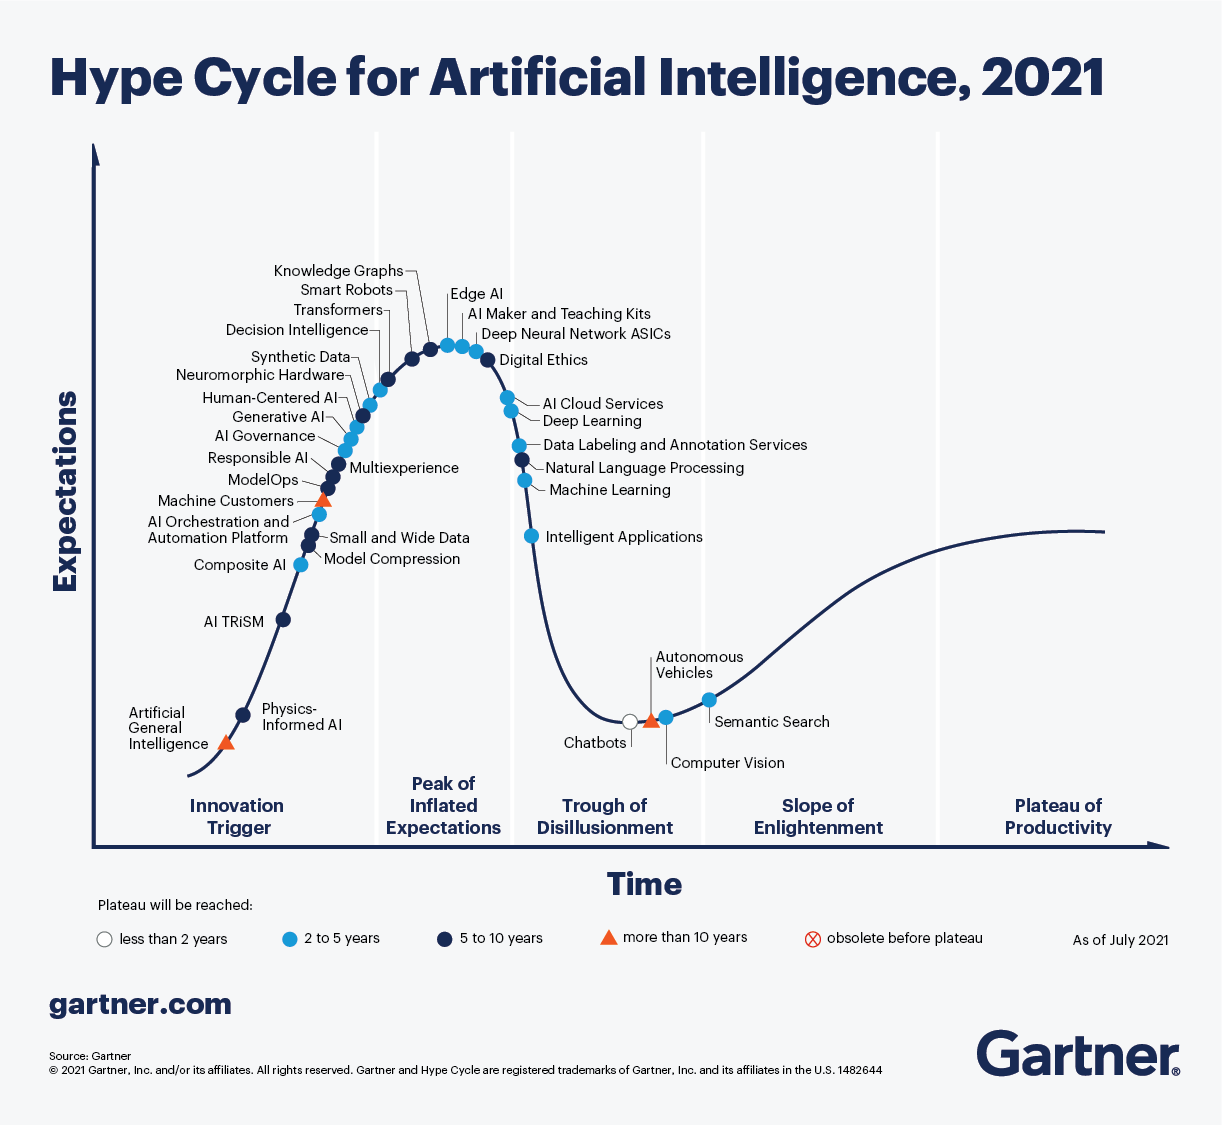
\includegraphics[width=\linewidth]{figures/Ch1/gartner-ai2021.png}
\caption{Hype Cycle for Artificial Intelligence 2021}
\label{f:gartner-ai2021}
\end{figure}

\section{Objectives}
\label{s:Objectives}
The research conducted in this dissertation aims to implement and experiment with different machine learning models to achieve a prediction of time series variables from an industrial field.


\textbf{General Objective:} Develop an intelligent system for industrial variables monitoring and forecasting.

\textbf{Specific Objectives:}

\begin{itemize}
\item Identify and characterize principal variables that carry out a proper forecasting.
\item Develop an intelligent system based on the key variables obtained and different forecasting models.
\item Evaluate each model performance to determine which model is suitable under different testing conditions.
\end{itemize}

\section{Thesis Question}
\label{s:Question}
The principal question addressed in this dissertation is:

¿How accurate can be predicted water quality parameters of an industrial wastewater treatment plant an intelligent system?

\section{Contributions}
\label{s:Contributions}

Our key contributions include:

\begin{enumerate}

  \item Machine Learning algorithms application in industrial scenarios. 
  
  \item Evaluation of different ensemble methods to improve single predictive models for industrial field.

\end{enumerate}

\section{Thesis Outline}
\label{s:Outline}

The remainder of this thesis is organized as follows. 

\begin{description}

  \item[Chapter \ref{c:Background}] presents background information relevant to the field of research. Provide details regarding topics and concepts the reader should know about wastewater treatment and data analysis computational techniques that will be mentioned throughout the thesis.
  
  \item[Chapter \ref{c:Related-Works}] provides a detailed discussion of the significant existing contributions to the field and how they relate to each other and the proposed intelligent system.
  
  \item[Chapter \ref{c:Contribution-1}] describes the properties and development process of the three machine learning approaches proposed. it details the considerations for all three model designs. Also, three different ensemble methods are proposed to improve the performance of each individual model.
  
  \item[Chapter \ref{c:Contribution-2}] provides some implementation details of the models and presents the results obtained for single models and ensemble ones. 
  
  %\item[Chapter \ref{c:Experiments}] details testing of the proposed intelligent system and each of its parts. A data-amount sensibility experiment is presented.
  
  \item[Chapter \ref{c:Conclusions}] concludes this thesis. First, it summarizes the work. Then, it highlights interesting aspects of the research and provides a thorough discussion of potential topics and areas concerning Machine Learning and Wastewater treatment that may be intriguing for future research activities. 
  
\end{description}



